% !TeX spellcheck = es_ES
\documentclass[arial,a4paper,print]{article}

\usepackage{amsmath}
\usepackage{helvet}
\usepackage{lipsum}
\usepackage{multirow}
\usepackage{array}
\usepackage{physics}
\usepackage[version=4]{mhchem}
\usepackage{epsfig}
\usepackage{amssymb}
%\usepackage{svrsymbols}
\usepackage{siunitx}
\usepackage{graphicx}
\usepackage{cancel}
\usepackage{float}
\usepackage{siunitx}
\usepackage{subcaption}
\usepackage[labelfont=sc, font={footnotesize, singlespacing}]{caption}
\usepackage[margin=2cm]{geometry}  

\renewcommand{\familydefault}{\sfdefault}

\usepackage[spanish]{babel}
%opening
\title{Química: Selectividad 2022}
\author{tomiock}

\begin{document}
	
\maketitle
	
\section{La radiación, los átomos y las moléculas}
\subsection{Radiación EM y interacciones entre átomos}
La radiación electromagnética se puede caracterizar mediante diversas magnitudes: 
\begin{enumerate}
	\item Longitud de onda ($\lambda$): \\
	Distancia mínima entre dos puntos en fase (mismo estado de vibración. 
	\item Periodo ($T$): \\
	El tiempo que tarda la onda en recorrer la longitud de onda. 
	\item Frecuencia ($\nu$): \\
	El número de longitudes de onda que pasan por un punto determinado en un segundo. Se puede relacionar con su longitud de onda y velocidad de propagación: 
	\begin{equation*}
			\nu = \frac{c}{\lambda}
	\end{equation*}
	En el caso de la radiación EM su velocidad de propagación es $c$, la velocidad de la luz, claro. 
\end{enumerate}
	
Se relacionan la energía con la longitud de onda y la frecuencia de la siguiente manera:
	\begin{equation*}
		E = h\frac{c}{\lambda} 
	\end{equation*}
	
\subsubsection{Radiación Infrarroja}
Los fotones ubicados en el espectro infrarrojo no tienen suficiente energía para poder provocar la transición electrónica de los átomos, pero si que los hacen vibrar. Cuando la radiación infrarroja es absorbida por los átomos estos usualmente pases de un estado de vibración a otro más energético, empiezan a vibrar de otra manera. Pueden o no pasar a un estado de vibración excitado. Más adelante veremos como se utiliza este fenómeno para determinar los grupos funcionales de substancias. 
	
\subsubsection{Espectro Visible}
En cambio cuando se absorben los fotones ubicados en el espectro visible, estos provocan saltos electrónicos, cuando un electrón pasa a estar en un orbital diferente con más energía.


Además conviene saber cuál es la relación entre la radiación IR y UV con el efecto invernadero y la capa de ozono.  
	
	
\subsection{Modelo atómico, Propiedades Periódicas de los Elementos y Cuantificación de la Energía} 

\subsubsection{Hipótesis de Planck}
La energía va en paquetes, osea cuantos de energía, de ahí viene la palabra cuántica, lo pillas?

También piensa en esta ecuación:
\begin{equation*}
	E = h\nu
\end{equation*}

No tengo nada más que decir.

\subsubsection{Modelos de los átomos}
Hay una nube de probabilidades a la cual llamamos orbital. Hay varios tipos de orbitales que están organizados según la energía que tienen. Hay que recortad que están organizados discretamente, no hablamos de un intervalo continuo de energía. 

Los orbitales se describen a partir de los números cuánticos asociados a un elemento:
\begin{enumerate}
\item N. Cuántico Principal $n$:\\
Describe lo grande que es un orbital. Es un número natural (sin cero), $n\in\mathbb{N}$. 

\item N.C. Secundario $l$:\\
Describe la forma del orbital, puede tener 4 valores:
\begin{align*}
	l = 0 \rightarrow \text{orbital } s \\
	l = 1 \rightarrow \text{orbital } p \\
	l = 2 \rightarrow \text{orbital } d \\
	l = 3 \rightarrow \text{orbital } f 
\end{align*}

\item N.C. Magnético $m_{l}$:\\
La cantidad de números magnéticos que puede llegar a tener un electrón depende de los números Hay $\pm l$ números magnéticos. Por cada valor de $l$ los números magnéticos toman los valores $+l$ y $-l$. 

\item N.C. Spin $m_{s}$:\\
Nadie sabe lo que es el spin\footnote{Mi amigo que esta en tercero de física no quiere que ponga esto pero lo pongo igual, sin embargo, piensa que es un chiste.}. Pero este número esta relacionado con las propiedades magnéticas del electrón. Para cada número $m$ hay dos valores de $m_{s}$, concretamente $+\frac{1}{2}$ i $-\frac12$. 
\end{enumerate}

\subsubsection{Configuración Electrónica}
A partir del número de electrones que tiene un átomo, podemos saber su configuración electrónica. Esto se consigue a partir del diagrama de Moeller:
\begin{figure}[H]
	\centering
	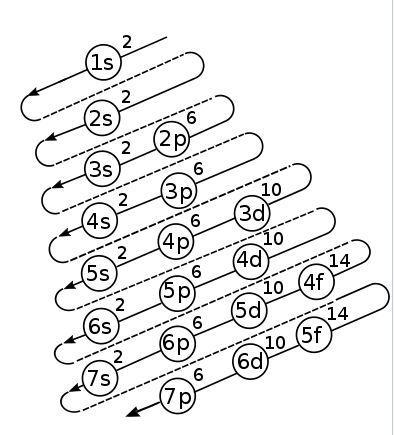
\includegraphics[width=0.2\linewidth]{figures/moeller}
	\caption{Diagrama de Moeller, las flechas indican la dirección hacia donde hay que ir para que al añadir un electrón se vaya al siguiente orbital.}
	\label{fig:moeller}
\end{figure}

Por ejemplo la configuración del sodio ($\ce{Na}, z=11$):
\begin{equation*}
	\ce{Na} (z=11): \ce{1s^{2} 2s^{2} 2p^{6} 3s^1}
\end{equation*}

A partir del último orbital se puede saber la posición del elemento en la tabla periódica, o hacer el camino inverso y averiguar la configuración electrónico a partir de la posición en la tabla. A partir de la configuración del sodio anterior podemos saber que está en $(3,1)$, es decir, en el tercer período en la primera columna. 

El número $n$ del orbital indica el período en el que se encuentra, mientra que el número $l$ (la letra) junto al superíndice, indica la columna. También con la letra del número $l$ podemos saber su posición entre los cuatro grandes grupos de la tabla periódica:
\begin{figure}[H]
	\centering
	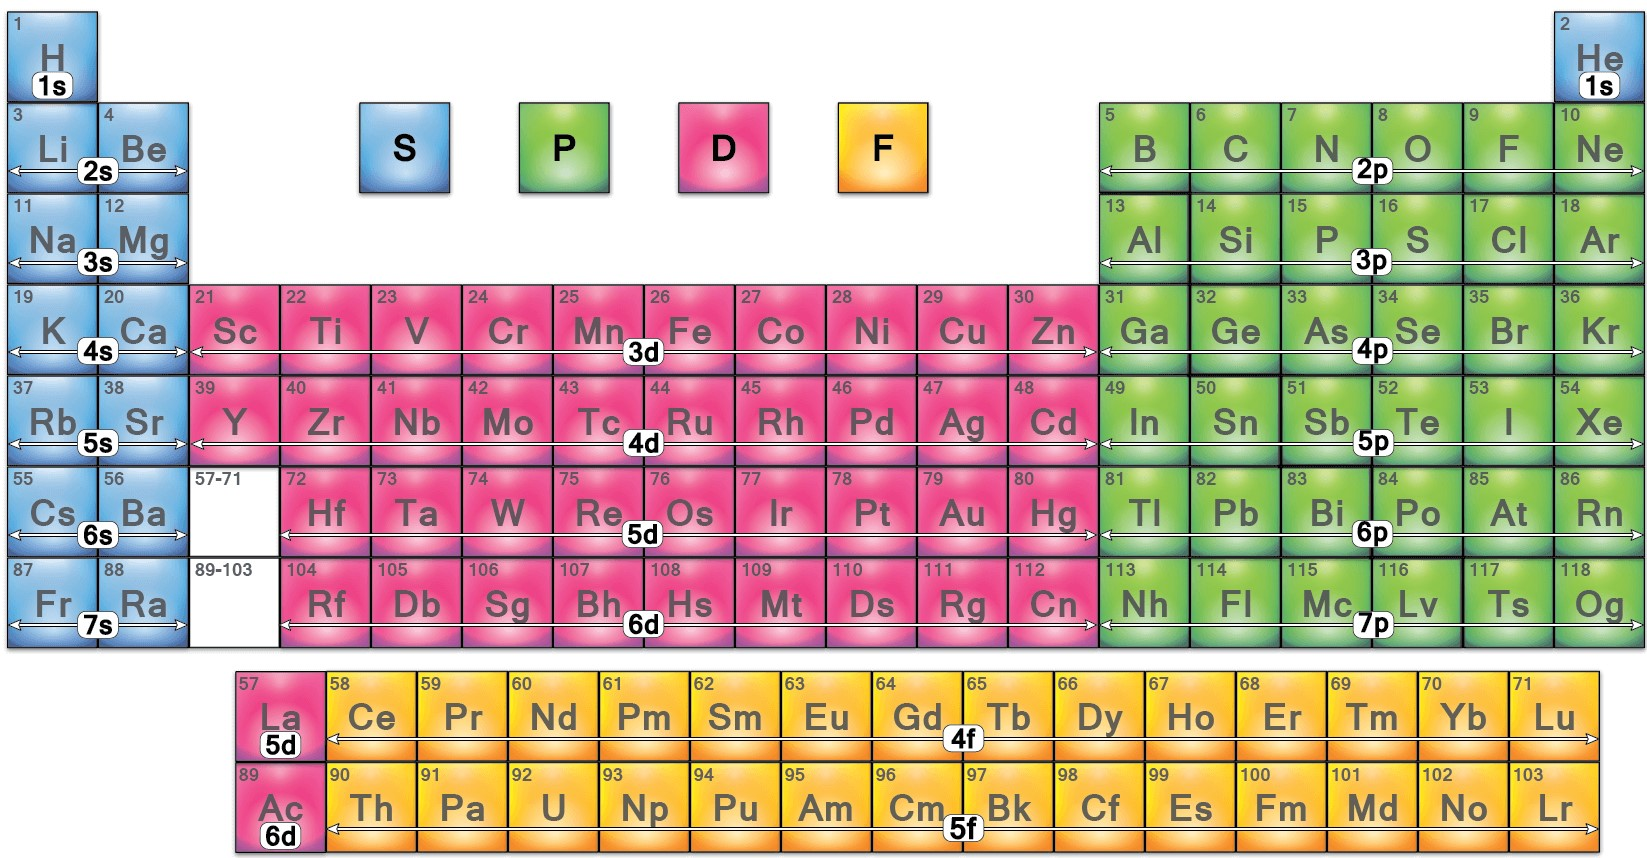
\includegraphics[width=0.8\linewidth]{figures/ptable_orbitals.png}
	\caption{Tabla periódica con la configuración electrónica de cada elemento (el último orbital). }
	\label{fig:ptableorbitalspng}
\end{figure}

\subsubsection{Periodicidad de las Propiedades de los Átomos}
Dependiendo de donde esté colocado un elemento en la tabla periódica podemos saber cualitativamente alguna de sus propiedades o lo podemos compara cualitativamente con otro elemento (decir si una propiedad es mayor o menor en relación a otro elemento). Para ello se empieza sabiendo la ubicación que tiene en la tabla periódica, usualmente en los ejercicios la posición se tiene que calcular a partir de la la configuración electrónica como ya he enseñado antes.  

Las propiedades que se pueden relacionar con la posición de la tabla periódica son las siguientes:
\begin{itemize}
	
\item \textbf{Energía Ionización $E_{i}$}:\\
Es la energía necesaria para arrancar un electrón de la capa de valencia de un átomo en estado fundamental y en fase gaseosa:
\begin{equation*}
	\ce{X_{(g)} \xrightarrow{E_{i}}}X^{+}_{(g)} + e^{-}
\end{equation*}

La cantidad de $E_{i}$ se determina a partir de estos factores:
\begin{itemize}

\item Proximidad entre el electrón y el núcleo:\\
A más proximidad (menos $n$) más $E_{i}$.

\item Carga nuclear que atrae a los electrones:\\
Cuanta más carga positiva más fuerza y más $E_{i}$.

\item Apantallamiento que hacen los electrones interior al exterior:\\
Cuanto más lejos esté un electrón más apantallamiento harán los electrones entre este y el núcleo, por lo tanto menos es la $E_{i}$.

\end{itemize}
Estos factores se pueden resumir en la ubicación del elemento de tal manera:
\begin{itemize}

\item Mismo grupo:\\
Cuanto menor sea el período (más arriba) más cerca del núcleo se encuentra y por lo tanto mayor $E_{i}$. 

\item Mismo período:\\
Dentro de un mismo período, los elementos están al mismo nivel energético y por lo tanto lo que hace variar su $E_{i}$ es cuanta carga esté en el núcleo, entonces, cuanto más a la derecha se encuentre (mayor grupo) más $E_{i}$ tendrán debido a que aumenta la cantidad de protones en el núcleo. 

\end{itemize}

Pueden haber una segunda o tercera energía de ionización, pero no será cuando se arranca un electrón de un átomo en un estado fundamental, sino un anión con carga $-1$ o $-2$, dependiendo si es la segunda o la tercera. Al saber la configuración electrónica del ion se podrá saber si su energía de ionización disminuye mucho o poco. Si al arrancar el primer electrón, no el $n$ del electrón siguiente, no habrá una gran variación en la segunda $E_{i}$. 

\item \textbf{Afinidad Electrónica}:\\
Es el cambio de energía que se produce cuando un átomo neutro en estado gaseoso captura un electrón y se forma un anión:
\begin{equation*}
	\ce{X_{(g)} + e^{-} \rightarrow X^{-}_{(g)}}
\end{equation*}
Al ser un proceso exotérmico en la muy amplia mayoría de los elementos, la afinidad electrónica suele tener signo negativo. 

Viene determinada por estos factores:
\begin{itemize}

\item La proximidad entre el electrón captado y el núcleo:\\
Cuando más cerca, más atracción y más energía se desprende en el proceso.

\item La carga nuclear:\\
Cuanta más carga (mayor $Z$) más atracción y más energía se desprende. 

\item Apantallamiento de los electrones:\\
Cuando más lejos este el electrón, más electrones de por medio y menos atracción. Este factor altera muy poco la afinidad. 
\end{itemize}

Cuando se combinan, tenemos que:
\begin{itemize}
\item Mismo grupo: \\
Cuanto más arriba (menor período), más cerca del núcleo se encuentra y menos apantallamiento hay, por lo tanto aumenta la afinidad electrónica. 

\item Mismo período: \\
Cuanto más a la derecha (mayor grupo) más carga hay en el núcleo, y más energía se libera al captar el electrón. 

\end{itemize}

\item \textbf{Electronegatividad}:\\
La electronegatividad $E_{n}$ es la forma de medir la tendencia de un átomo a atraer electrones cuando se combina formando una molécula. 

Esta propiedad no tiene unidades. Al igual que la afinidad electrónica y la energía de ionización, aumenta de abajo a arriba y de izquierda a derecha (es más fuerte arriba y a la derecha). 

Sin embargo, no aumenta de forma constante, suelen haber saltos grandes de un elemento a otro y incluso a veces disminuye en contra de la regla dicha anteriormente. El caso más notable es el hidrógeno que tiene una muy alta para estar en el primer grupo. 

\item \textbf{Energía Reticular de un Compuesto Iónico}:\\
Es la energía almacenada dentro de un compuesto iónico, se adquiere al formarlo. Es la energía que se desprende cuando se forma un mol de compuesto iónico a partir de sus iones a distancia infinita y estado gaseoso.

Este concepto se desarrollará más adelante en el tema de termodinámica. 

\item \textbf{Volumen atómico}:
Va a la par con el radio. 

\item \textbf{Radio Atómico}:
Es la mitad de la distancia entre los núcleo de dos átomos de un mismo elemento formando una molécula diátomica, una estructura covalente o estructura con enlace metálico. 

Según la posición en la tabla periódica podemos decir que:
\begin{itemize}
	
	\item Mismo Grupo:\\
	El radio aumenta de arriba a abajo (mayor período, más radio), porque aumenta el número cuántico principal, que hace aumentar la distancia del orbital al núcleo, y por lo tanto el radio. 
	
	\item Mismo Período:\\
	Va aumentando de derecha a izquierda (menor grupo, más radio), esto es porque al aumentar la carga del núcleo hay una disminución en la atracción electrón-núcleo y por lo tanto en la distancia. 
	
	Hay que decir que cuando se pasa de un elemento en estado fundamental a un ion, su radio puede cambiar debido al cambio en el número de electrones, al hacer que hayan menos (catión) hay menos repulsión entre ellos y se da lugar una contracción. Debido a que se reduce el volumen, también lo hace el radio. 
	
	En el caso de los aniones, al haber un electrón más, aumenta la repulsión entre los electrones y por lo tanto el átomo se más grande, aumentando el volumen y el radio. 
	
	La clave es pensar que los electrones se repelen entre ellos por tener la misma carga y esto afecta al tamaño del átomo. 
	
\end{itemize}


\end{itemize}



\subsection{Espectroscopia}
A través de mirar a algún tipo de espectro que surge a través de propiedades atómicas o moleculares, podemos identificar sustancias. 

\subsubsection{Espectroscopia IR}
La espectroscopia basada en la radiación infrarroja consiste en mirar el espectro de absorción de una sustancia en concreto con tal de identificarla.  

Debido a que una molécula aborde IR que tiene el efecto de cambiar su estado vibracional, podemos asociar grupos funcionales (tipos de enlaces) a picos en un espectro de transmitancia de IR de una molécula. 

En los ejercicios va a haber un gráfico parecido a este:
\begin{figure}[H]
	\centering
	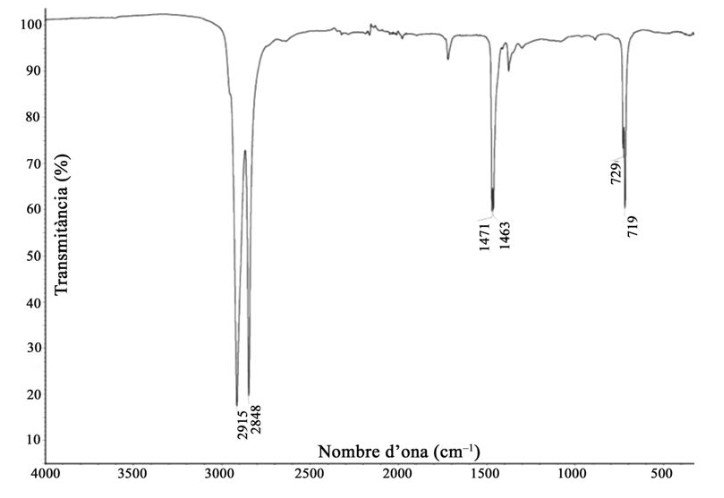
\includegraphics[width=0.5\linewidth]{figures/IR}
	\caption{Ejemplo de gráfico con espectro IR de una molécula}
	\label{fig:ir}
\end{figure}

Los picos que se pueden ver están asociados a enlaces/grupos funcionales, normalmente la correlación entre picos y enlaces se muestra mediante esta tabla:
\begin{figure}[H]
	\centering
	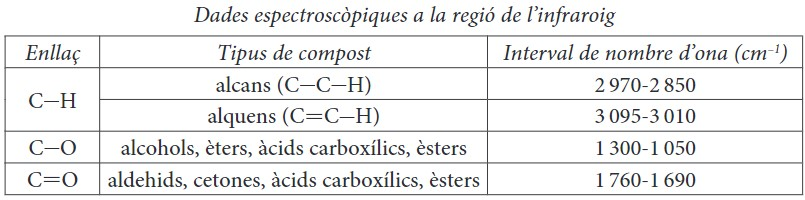
\includegraphics[width=0.7\linewidth]{figures/tabla_IR}
	\caption{Tabla en la que se muestran los enlaces y sus correspondientes picos.}
	\label{fig:tablair}
\end{figure}

Para realizar los ejercicios de este punto, hay que saber cuales son las magnitudes que se encuentran en cada eje. En el horizontal esta el número de onda $\tilde{\nu}$ que es la inversa de la longitud de onda $\tilde{\nu} = \frac{1}{\lambda}$. En el vertical está la transmitancia, el porcentaje de lo absorbido respecto a lo transmitido. Igualmente no es necesaria una definición de este concepto.  Pero si que lo es una pequeña explicación de como sucede, en la cual hay que mencionar los estados de excitación de vibración de las moléculas.  

\subsubsection{Resonancia magnética nuclear (RMN)}

Este tipo de espectroscopia funciona a partir de la orientación de los núcleos atómicos dentro de un campo magnético. Los núcleos pueden tener dos tipos de orientaciones (en sentido del campo $\vec{B}$ o en el contrario) las cuales tienen diferentes niveles de energía (estados de energía). Estos estados pueden tener transiciones entre ellos que son detectables en el campo magnético. La frecuencia de estas transiciones dependen del propio núcleo y del entorno que tiene (cantidad de enlaces). Usualmente se utiliza la RMN de protones $ \ce{H^{1}_{1}} $ la cual nos dice. 

Una RMN mide el desplazamiento químico entre un núcleo de hidrógeno respecto al patrón tetrametilsilano (TMS): 
\begin{equation*}
	\delta(\text{ppm}) = 10^{6}\frac{\nu_{\text{muestra}} - \nu_{\text{referencia}} }{\nu_{\text{referencia}} }
\end{equation*}

El desplazamiento $\delta$ está en un rango de $0$ a $12$. Es una medida que nos dice como de parecidos son los hidrógenos según su entorno. Concretamente sobre la distancia (número de enlaces) a los que están un par de hidrógenos. Aquí hay un ejemplo de un espectro con una explicación para interpretarlo:
\begin{figure}[H]
	\centering
	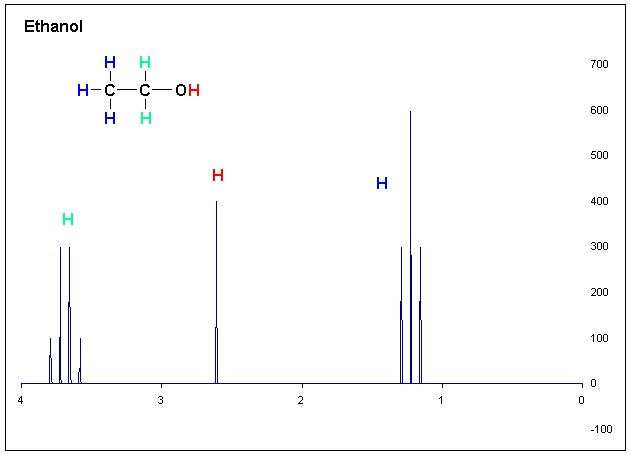
\includegraphics[width=0.5\linewidth]{figures/RMN}
	\caption{Los hidrógenos verdes solo 'detectan' a los azules ya que están enlazados a un carbono y a tres enlaces de distancia (los cuatro picos más a la izquierda). Los picos siempre van a ser una más que los carbonos del mismo tipo que se detectan. Podemos ver como el hidrógeno rojo solo generar un pico (él mismo), ja que no 'detecta' a ninguno otro porque no está enlazado a un carbono. Finalmente los azules solo detectan a lo dos verdes (por eso tres picos), también sus picos serán más altos debido a que más hidrógenos los generan (tres de ellos comparado con los 2 de los verdes).}
	\label{fig:rmn}
\end{figure}

Resumidamente:
\begin{itemize}
\item Solo se detectan hidrógenos entre si cuando hay carbonos de por medio y están a tres o menos enlaces de distancia. 

\item Los hidrógenos que están enlazados al mismo carbono se detectan entre ellos de forma que forman picos de mayor intensidad. 

\item Asimismo si los hidrógenos detectan a varios hidrógenos de un mismo entorno, el pico que forman es mayor en intensidad. 

\item Los picos tendrán están en grupos de $n+1$ hidrógenos detectados. 

\end{itemize}

\subsubsection{Espectrometro de masas}	
En esta técnica de identificación de sustancias, estas de vaporizar de forma que liberan cationes que pueden ser detectados para analizar su masa y de esta manera averiguar de que sustancia se trata. Para obtener los fragmento, se vaporiza la sustancia y es bombardeada con un flujo de electrones para poder obtener los cationes (fragmentos con carga positiva de la sustancia). Estos se detectan de tal manera que podemos saber tanto su masa como la cantidad de ellos que hay, de esta manera obtenemos una gráfica como esta:
\begin{figure}[H]
	\centering
	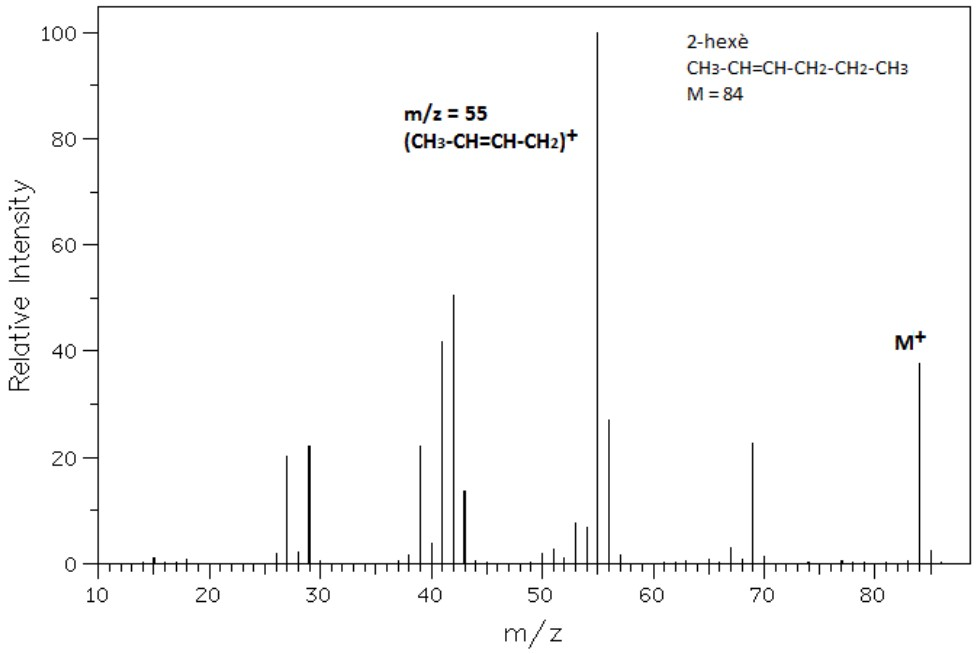
\includegraphics[width=0.5\linewidth]{figures/espec_masa}
	\caption{Espectrometro de masas del 2-hexeno. Podemos ver como el ion molecular $\ce{M^}$ con una masa de 84 es el primer pico. El más alto es el de masa 55 que coincide con $\ce{CH_3-CH=CH-CH_2}$}
	\label{fig:especmasa}
\end{figure}

\pagebreak
En todos los espectros de este tipo hay un pico que corresponde al ion molecular, que es simplemente la molécula analizada pero con carga positiva. Usualmente es el pico con más masa, pero es común observar un pico con un hidrógeno debido a que este se fusiona al ion molecular durante el bombardeo de electrones. No obstante, el pico del ion molécula suele ser mucho más alto, y por lo tanto más reconocible. 

Los puntos de ruptura más comunes son:
\begin{itemize}
\item Hidrocarburos: enlaces sencillos tipo $\ce{C-C}$
\item Alcoholes, aminas y éteres: carbono junto al nitrógeno/oxigeno y carbono siguiente.
\item Ésters, aldehidos y cetonas: carbono del grupo carbonilo y el átomo siguiente.
\end{itemize}

Usualmente se compara entre dos gráficas o se tiene que justificar la relación entre una gráfica y una molécula. En ambos casos conviene mirar al ion molecular para saber si la gráfica tiene que ver algo con la molécula. 

\subsection{Gases}

\subsubsection{Temperatura y $E_{k}$}
Existe una relación entre la temperatura de un gas y la energía cinética media de sus partículas $E_{k}$. Intuitivamente podemos ver que es una relación directamente proporcional lineal. Cuando una és más grande, la otra también. 

La energía cinética media de un gas es:
\begin{equation*}
	\overline{E_{k}} = \frac32 kT
\end{equation*}
Donde $k$ es la constante de Boltzmann ($1.38\cross10^{-23}\si{J/K}$) y $T$ la temperatura en Kelvin. 

\subsubsection{Velocidad de Difusión}
Definimos velocidad de difusión como la velocidad a la cual un gas se distribuye uniformemente por el espacio. 

La Ley de Graham nos dice que esta velocidad es inversamente proporcional a la raíz cuadrada de su densidad (comparando dos gases distintos):
\begin{equation*}
	\frac{v_{1}}{v_{2}} = \frac{\sqrt{d_{2}}}{\sqrt{d_{1}}}
\end{equation*}
\begin{equation*}
	\frac{v_{1}}{v_{2}} = \frac{\sqrt{\frac{m_{2}}{V_{2}}}}{\sqrt{\frac{m_{1}}{V_{1}}}}
\end{equation*}
Debido a que los volúmenes son los mismo $V_{1} = V_{2}$, finalmente tenemos que:
\begin{equation*}
	\frac{v_{1}}{v_{2}} = \frac{\sqrt{m_{2}}}{\sqrt{m_{1}}}
\end{equation*}


\subsubsection{Modelo de los Gases}

¿Por que hay una diferencia entre la ley de los gases ideales $pV = nRT$ y su comportamiento real?
Para ello hemos de mirar en que se basa el modelo de los gases ideales:
\begin{itemize}
\item Están formados por partículas que se mueven constantemente.
\item El tamaño de las partículas es negligible comparado con el volumen del recipiente. 
\item Las fuerzas de atracción/repulsión entre las partículas son negligibles. 
\item Los choques entre partículas son perfectamente elásticos. 
\item A la mismo temperatura, la $\overline{E_{k}}$ de las partículas se mantiene constante. 
\end{itemize}

A partir de estos principios y pensando (no se como) podemos llegar a estas conclusiones:
\begin{itemize}
\item A altas presiones, el tamaño de las partículas es considerable frente al volumen del recipiente. 
\item Las fuerzas de atracción entre las moléculas no se pueden ignorar.
\end{itemize}

\subsubsection{Licuación de un gas}
Cuando se comprime un gas lo suficiente es posible que este pase a estar en fase líquida. Pero para que esto pase la temperatura ha de estar por debajo del punto crítico (en el diagrama de fases). Por arriba de la temperatura crítica es imposible licuidar un gas. El punto crítico es el que se encuentra arriba a la derecha en los diagramas de fase. En este punto, la sustancia se debe de considerar un gas y un líquido al mismo tiempo.
\begin{figure}[H]
	\centering
	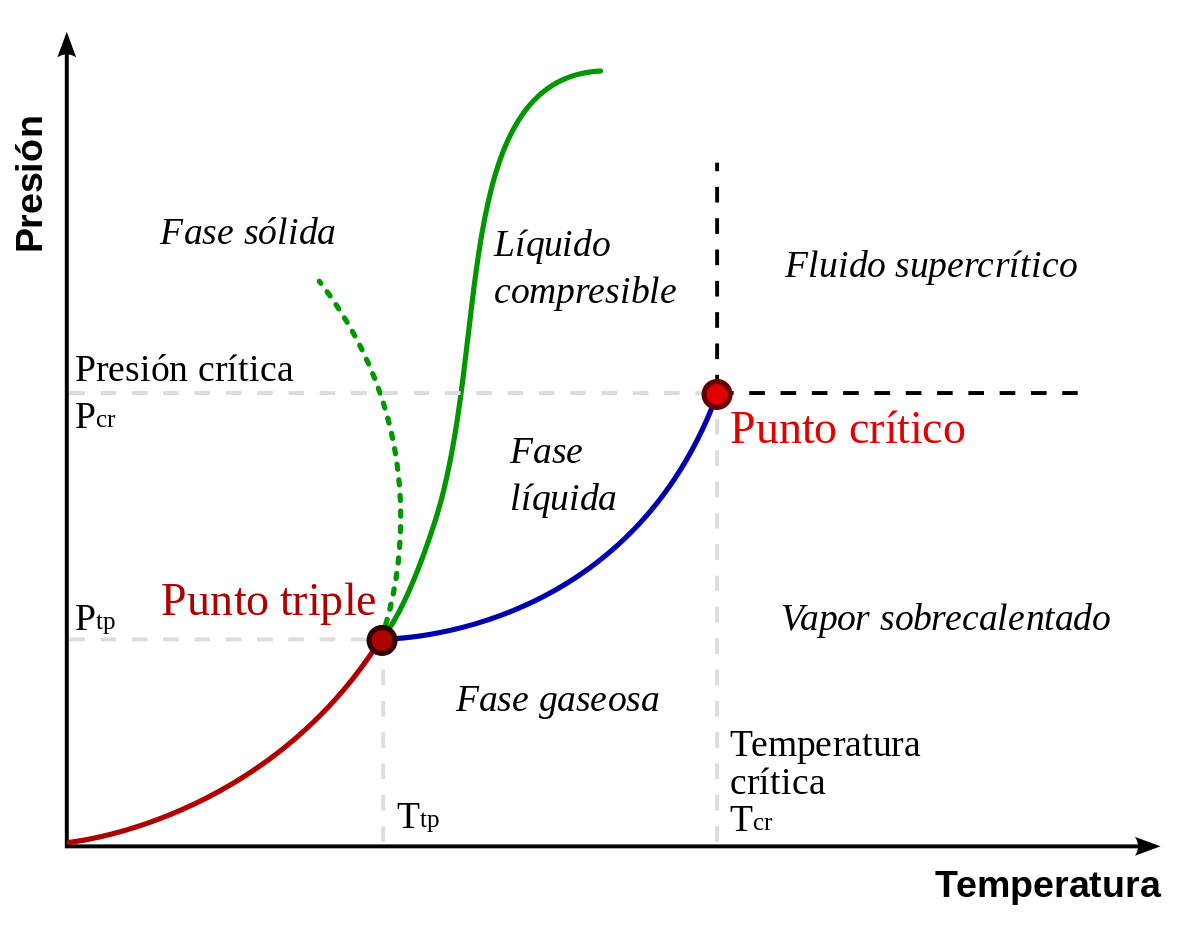
\includegraphics[width=0.5\linewidth]{figures/diagrama_fases}
	\caption{En este diagrama se pueden ver el punto crítico arriba a la derecha, junto a la zona donde el fluido está en estado supercrítico. Solo para las temperaturas por debajo de la temperatura supercrítica $T_{\text{cr}}$ se puede licuidar el gas. }
	\label{fig:diagramafases}
\end{figure}

\section{Los cambios de energía en las reacciones químicas}

\subsection{Importancia de saber esto}
Saber esto (esta sección) de los apuntes es muy importante porque asi podemos saber la cantidad de energía que generan diversas reacciones para de esta manera tener procesos industriales más eficientes. Esto es especialmente útil cuando hablamos de las reacciones de combustión de compuestos orgánicos. 

\subsection{Energía Interna y Entalpía}
\subsubsection{Energía Interna}
La suma de todas las energías que (cinética, potencial, vibratoria...) que forman parte de una sustancia se denomina energía interna. Esta energía solo se transferir al entorno en forma de calor o trabajo. Para entender este concepto a escala microscópica podemos pensar en la suma de las energías de una o varias partículas. 

La variación de energía interna $\Delta U$ de un sistema es igual a la calor $Q$ y el trabajo $W$ sumados:
\begin{equation*}
	\Delta U = Q + W
\end{equation*}
Donde está definida a partir de la variación de temperatura $\Delta T$ y la calor especifica $C_{e}$ de una sustancia, junto a la masa de la muestra que trasfiere esa calor:
\begin{equation*}
	Q = mC_{e}\Delta T
\end{equation*}

Y el trabajo como:
\begin{equation*}
	W = -p_{\text{ext}}S\Delta x = F_{\text{ext}}\Delta x
\end{equation*}
Donde $-p_{\text{exp}}$ es la presión externa y $S$ es la superficie donde actúa la fuerza $F_{\text{ext}}$ que desplaza un cuerpo una distancia de $\Delta x$. En este caso, consideramos que la fuerza está definida por la presión y la superficie a la cual se aplica $F=pS$. 

Podemos ver como en una reacción en la cual el volumen es constante $\Delta V$, la única forma en la que puede variar la energía interna es a través de la calor:
\begin{equation*}
	\Delta U = Q_{v}
\end{equation*}
En toda reacción a volumen constante, la variación de energía interna solo es causada por la transferencia de calor durante el proceso. 

\subsubsection{Entalpía}
La entalpía es la suma de la energía interna y $pV$:
\begin{equation*}
	H = U + pV
\end{equation*}

A partir de la definición de la energía interna, podemos ver que en una reacción a presión constante, la única manera de transferir calor coincide con la variación de la entalpía:
\begin{equation*}
	\Delta H = Q_{p}
\end{equation*}
Con ella, podemos saber si una reacción es exotérmica (libera calor) o endotérmica (absorbe calor):
\begin{align*}
	\Delta H < 0 \text{ proceso exotérmico} \\
	\Delta H > 0 \text{ proceso endotérmico}
\end{align*}

También podemos ver como para todas las reacciones entre gases en las cuales los moles de productos y reactivos no varia, la entalpía y energía interna son iguales:
\begin{align*}
	Q_{p} = Q_{p} \\ \Delta H = \Delta U
\end{align*}

Podemos determinar la variación de la entalpía de una reacción como la resta de la entalpía de formación de sus productos con la de sus reactivos:
\begin{equation}
	\Delta H_{r} = \sum n_{p}\Delta H_{fp} - \sum n_{r}\Delta H_{fr}
\label{delta_H}
\end{equation}
Esta fórmula es que usualmente se tiene que utilizar para calcular la entalpía de una reacción con los datos que te dan sobre las entalpias de formación de las sustancias que forman parte de la reacción. 

\subsubsection{Experimento para determinar Entalpía/Energía Interna}

Concretamente se ha de conocer la determinación experimental de la calor de una reacción. A 
continuación hay un fragmento de una corrección de uno de estos ejercicios:

\line(1,0){450}

\textbf{Procediment experimental per determinar $\Delta H$ d'una dissolució:}
\\

En un \underline{calorímetre} hi col·loquem \underline{un determinat volum d’aigua} (o \underline{una determinada
massa d’aigua}) i mesurem la \underline{temperatura inicial}. Posteriorment, afegim una
\underline{determinada massa de NH4NO3 sòlid al calorímetre}. Agitem ràpidament la mescla per
dissoldre tot el sòlid, tapem el calorímetre i esperem un temps fins que la temperatura
que ens marca el termòmetre deixi de baixar (s’estabilitzi). Mesurem aquesta
\underline{temperatura final}.
\\

\underline{Material}:
\begin{itemize}
\item Calorímetre (per exemple un vas de plàstic amb tapa i aïllat).
\item Termòmetre.
\item Balança (i pipeta o proveta si \underline{mesurem el volum d’aigua}).

\end{itemize}


\underline{Mesures experimentals que necessitem}:
\begin{itemize}
\item Massa de NH4NO3 i massa o volum de l’aigua.
\item Temperatura inicial de l’aigua, i temperatura final de la solució una vegada s’ha
estabilitzat.
\end{itemize}


\underline{Altres dades que necessitem per calcular la $\Delta H$ de la dissolució}:
\begin{itemize}
\item Capacitat calorífica de la solució 
\end{itemize}

\line(2,0){450}
\\
Lo más importante es tener en cuenta se da lugar la reacción, es decir, como la ponemos en marcha por así decirlo. Porque todo lo otro será igual para cualquier medida de la calor que se haga, sin importar la reacción (e.g. medida de la temperatura final y inicial). 
\pagebreak
\subsubsection{Relación entre entalpía y energía interna}

Simplemente se ha de saber que cuando es una reacción a volumen constante, se ha de calcular al variación en energía interna $\Delta U$ y cuando es una reacción a presión constante, se ha de calcular la entalpía $\Delta H$. 

También tengo que decir que hay varios tipos de entalpía:
\begin{itemize}
\item Entalpía Reacción: Calor que libera una reacción al suceder. Se calcula con la fórmula \ref{delta_H}. 

\item Entalpía Formación: Energía necesaria para formar un mol de producto. Para las sustancias puras, es $0\,\si{J/mol}$. 

\item Entalpía Combustión: Es la entalpía de reacción pero para una combustión. Son todas negativas, ya que son exotérmicas. 
\end{itemize}

\subsection{Ley de Hess, Diagramas de Entalpias}

\subsubsection{Ley de Hess}
Tiene mucha lógica esto, esta ley dice que se pueden encadenar las reacciones pensando que una reacción es como una suma algebraica. Por ejemplo, una reacción expresada como una suma algebraica de otras reacciones, tiene una entalpía que es la suma algebraica de las entalpias de las otras reacciones. 

En otras palabras:
\begin{equation*}
	A \rightarrow B; \, B \rightarrow C; \, C\rightarrow D
\end{equation*}
\begin{equation*}
	A \rightarrow B \rightarrow C \rightarrow D
\end{equation*}

\subsubsection{Diagramas de Entalpias}
Normalmente la entalpía de una reacción se puede expresar con los siguientes diagramas:
\begin{figure}[H]
	\centering
	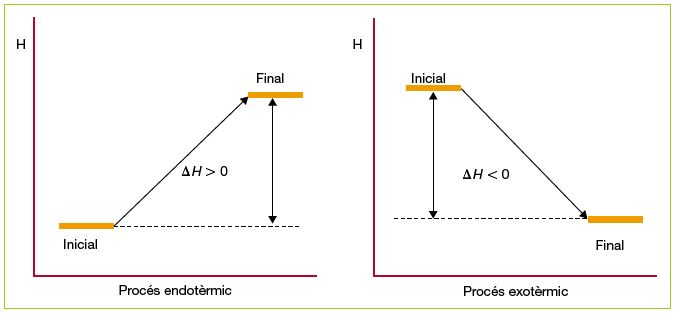
\includegraphics[width=0.5\linewidth]{figures/diagrama_H}
	\caption{En estos dos diagramas, se puede ver como el primero es endotérmico y el segundo exotérmico.}
	\label{fig:diagramah}
\end{figure}
Pueden llegar a complicarse mucho como este de aquí:
\begin{figure}[H]
	\centering
	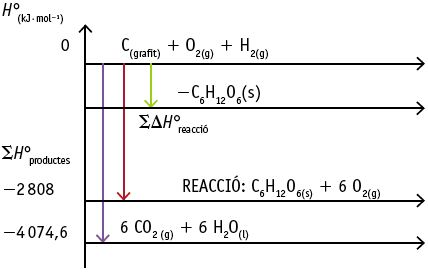
\includegraphics[width=0.5\linewidth]{figures/diagrama2_h}
	\caption{Diagrama de entalpias usando la Ley de Hess. La reacción es $\ce{C_{6}H_{12}O_{6} + 6O_{2}\rightarrow 6CO_{2} + 6H_{2}O}$. En este caso se calcula primero la entalpía de formación del \ce{C_{6}H_{12}O_{6}}, para luego calcular la entalpía de la reacción.}
	\label{fig:diagrama2h}
\end{figure}
\pagebreak

\subsection{Entalpía de Enlaces}
En las reacción se rompen y forman enlaces, y pues tiene sentido que haya una energía asociado a la rotura de los enlaces, a esta energía la llamamos Entalpía de Enlace. 

Podemos definir la entalpía de una reacción a partir de la entalpía de los enlaces:
\begin{equation*}
	\Delta H^{\circ}_{\text{reacción}} = \sum \text{Energía enlaces rotos} - \sum\text{Energía enlaces formados}
\end{equation*}

Intuitivamente se pueden ver de que factores depende la energía/entalpía de un enlaces: 
\begin{itemize}
\item La longitud afecta inversamente, cuando más lejos, más débil es
\item Si es un enlace covalente, el carácter que tiene afecta a la energía (simple, doble, triple)

\end{itemize}

\subsection{Entalpía Reticular Iónica}
Como ya he dicho antes, es la energía que se desprende cuando se forma un mol de compuesto iónico a partir de sus iones a distancia infinita y estado gaseoso.

Para entender como se calcula podemos mirar el ciclo de Born-Haber, que es el ciclo que la describe:
\begin{figure}[H]
	\centering
	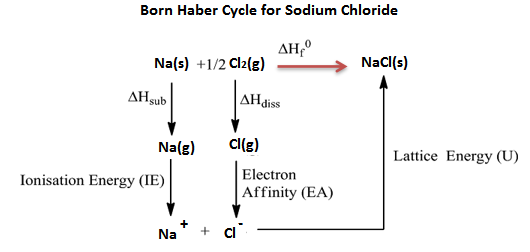
\includegraphics[width=0.6\linewidth]{figures/born-haber}
	\caption{Ciclo de Born-Haber que describe la energía reticular del cloruro de sodio $\ce{NaCl}$, la sal de toda la vida. }
	\label{fig:born-haber}
\end{figure}

Debido a que empezamos con una sustancia sólida (el sodio) y la tenemos tener en estado gaseoso, tenemos que sublimarla (con $\Delta H_{\text{sub}}$), también necesitamos un átomo de cloro que al principio se encuentra en estado gaseoso diátomico ($\ce{Cl_2}$), por lo tanto tenemos que disasociarlo ( con $\Delta H_{\text{diss}}$). A causa de que tiene que reaccionar en forma de iones ($\ce{Na^+ + Cl^-}$) tenemos que ionizar el sodio y cloro con la energía de ionización ($E_{i}$) y la afinidad electrónica ($E_{af}$), respectivamente.  

Al mirar el ciclo podemos ver que la energía reticular se puede calcular con esta formula:
\begin{equation*}
	E_{\text{reticular}} = \Delta H^{\circ}_{f} - \left(\Delta H_{\text{sub}} + \Delta H_{\text{diss}} + E_{i} + E_{af}\right)
\end{equation*}

Calcularla en un ejercicio es muy fácil porque te dan los datos que necesitas (recuerda que tienen que ser 4 energías distintas por si acaso) pero si que hay que tener en cuenta como se pone la resta en la ecuación, pero recordando como se expresa la entalpía de formación es muy fácil averiguarlo:
\begin{equation*}
	\Delta H^{\circ}_{f} = E_{\text{reticular}} + \Delta H_{\text{sub}} + \Delta H_{\text{diss}} + E_{i} + E_{af}
\end{equation*}

\pagebreak
\section{Los Equilibrios de Fase y Equilibro Químico}

\subsection{Equilibrios y Diagramas de Fase}
Como ya sabemos, una sustancia se puede encontrar en diversas fases dependiendo de la temperatura y presión a la que esto, este fenómeno se representa muy bien en diagramas de fase como este:
\begin{figure}[H]
	\centering
	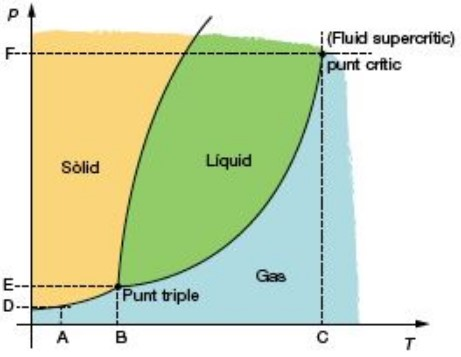
\includegraphics[width=0.5\linewidth]{figures/diagrama_fase}
	\caption{Diagrama de fase del $\ce{CO2}$, podemos ver representados el punto triple y el punto crítico.}
	\label{fig:diagramafase}
\end{figure}

Lo más importante sobre estos diagramas es saber interpretarlos, la cual diría que es bastante fácil. Primero de todo tenemos que tener en cuenta que hay dos puntos 'especiales':
\begin{itemize}
\item Punto Triple: Un punto del diagrama en el cual a una determinada temperatura y presión, una sustancia está al mismo tiempo entre las tres bases. En otras palabras, hay un equilibrio de las tres fases. 

\item Punto Crítico: Punto en el cual la sustancia es un gas y un líquido al mismo tiempo. La temperatura asociada a este punto (temperatura crítica) es la temperatura máxima a la que puede existir esta sustancia en estado líquido. 
\end{itemize}
 
Para hacer los ejercicios hay que saber que nombre tienen los cambios de estados (sublimación, solidificación, vaporización, condensación...). Lo típico que se estudia en la ESO. También hay que saber construirlos (los del agua y dióxido de carbono, sobretodo) a partir de datos que te dan, o que los tienes que completar. 

\subsection{Equilibrio Químico}

Las reacciones pueden ser reversibles, y a veces pasa que tienen que llegar a un equilibrio químico en el cual los sigue habiendo una cantidad de reactivos (la reacción no es completa). Una de estas reacciones es por ejemplo:
\begin{equation*}
	\ce{2NO + O_2 <=> 2NO2}
\end{equation*}

En todas las reacciones de equilibrio se cumplen las siguientes condiciones:
\begin{enumerate}
\item Las reacciones directa y inversa son termodinámicamente posibles en determinadas condiciones.
\item Se llega al equilibrio cuando la reacción directa y inversa tienen la misma velocidad. 
\item El estado de equilibrio es dinámico (tanto los reactivos como productos pueden formarse en cualquier momento). Pero este hecho no es perceptible macroscópicamente. 
\item La temperatura marca las proporciones a las cuales están los productos y reactivos cuando están en equilibrio. A parte de estas hay otras condiciones que pueden afectar. 
\end{enumerate}

\subsubsection{Equilibrios Heteros y Homos}
Se llama equilibrio heterogéneo a un equilibrio en el cual hay sustancias en diversas fases de estado involucradas. Normalmente son disoluciones en las cuales la solubilidad del soluto (un de los reactivos usualmente) está determinada por un equilibrio químico. Este tipo de equilibrios los veremos más adelante. 

\subsubsection{Constantes de Equilibrio $K_{c}$ y $K_{p}$}

Para una reacción química reversible de tipo:
\begin{equation*}
	\ce{aA + bB <=> cC + dD}\,,
\end{equation*}
se puede definir una constante de equilibrio $K_{c}$\footnote{Los productos siempre van arriba, con los reactivos abajo.}:
\begin{equation*}
	K_{c} = \frac{[C]^{c}[D]^{d}}{[A]^{a}[B]^{b}}
\end{equation*}

También existe una constante de equilibrio de presión $K_{p}$, definida como:
\begin{equation*}
	K_{p} = \frac{p_{C}^{c}p_{D}^{d}}{p_{A}^{a}p_{B}^{b}}
\end{equation*}

Podemos ver como para sustancias gaseosas y a partir de la ley de los gases ideales, podemos definir concentración de un gas como:
\begin{equation*}
	\frac{n_{i}}{V} = \frac{p_{i}}{RT}
\end{equation*}
Si hacemos una proporción entre concentraciones de dos sustancias tenemos que:
\begin{equation*}
	\frac{n_{i}/V}{n'_{i}/V} = \frac{p_{i}}{p'_{i}}
\end{equation*}
Debido a que en un equilibrio las sustancias están con el mismo volumen y las concentraciones están en cocientes, finalmente podemos definir una constante de equilibrio que depende de las presiones parciales de los compuestos involucrados en el equilibrio:
\begin{equation*}
	K_{p} = \frac{p_{C}^{c}p_{D}^{d}}{p_{A}^{a}p_{B}^{b}}
\end{equation*}

Conviene saber como calcular estas constantes para reacciones como las de la formación del amoniaco, la reacción de descomposición del carbonato de calcio y una reacción de esterificación. 

\subsection{Cocientes de Equilibrio $Q_{c}$ y $Q_{p}$}

Para un momento concreto con unas concentraciones en concreto existe un cociente de equilibrio $Q_{c}$ que determina como de cerca están estas concentraciones de llegar al equilibrio:
\begin{equation*}
	Q_{c} = \frac{[C]^{c}[D]^{d}}{[A]^{a}[B]^{b}}
\end{equation*}
Podemos ver que es igual que la constante en cuanto a su cálculo, pero lo que importa es que es lo que significan las concentraciones, si son las que están en equilibrio. La cuestión es esta:
\begin{itemize}
\item $Q_{c} < K_{c}$:\\
La reacción se da en el sentido directo, hacia la derecha.

\item $Q_{c} > K_{c}$:\\
La reacción se da en el sentido inverso, hacia la izquierda. 

\item $Q_{c} = K_{c}$:\\
Está en una situación de equilibrio. 
\end{itemize}

Como regla para memorizar: \\
La reacción va en sentido de la boca del tiburón (la boca es $<$), pero claro SIEMPRE hay poner la $Q_{c}$ primero y luego la $K_{c}$, esto grabado a grabado fuego (un tatuaje). 

\subsubsection{Cálculo con las constantes y los cocientes}

Se puede ver que a través de la $K_{c}$ y del cociente $Q_{c}$. Pero lo que es muy importante es hacer este tipo de esquemas/tablas:
\begin{figure}[H]
	\centering
	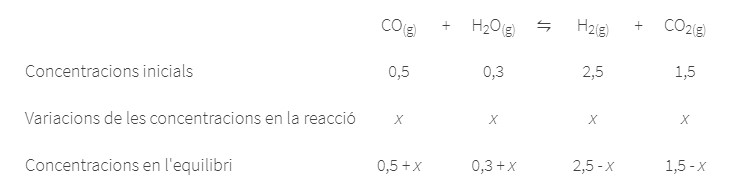
\includegraphics[width=0.7\linewidth]{figures/tabla_Kc}
	\caption{Tabla asociada a las concentraciones en un equilibrio de la reacción para la formación de dióxido de carbono. $x$ es la cantidad de concentración que varia una vez se llega al equilibrio. Se puede ver como los datos de la tabla variarían según cuales son las concentraciones iniciales. También hay que tener en cuenta las estequiometría implicada, porque los cocientes serían multiplicados por las concentraciones.}
	\label{fig:tablakc}
\end{figure}

Aunque usualmente, estas tablas se parecen más a esta:
\begin{figure}[H]
	\centering
	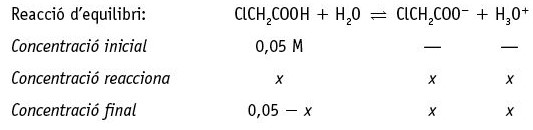
\includegraphics[width=0.7\linewidth]{figures/tabla2_Kc}
	\caption{En este caso podemos ver como se empieza solo con reactivos y al final hay una concentración $x$ para cada producto. Esta tabla corresponde a otro tema pero la he escogido como ejemplo. Ya se hablará de ella con más detenimiento en el futuro. }
	\label{fig:tabla2kc}
\end{figure}

\subsection{Factores que afectan a la constante de equilibrio}

\textbf{Ley de Le Châtelier}: \\
Lo mejor es entender este principio con estas tablas: \\


\begin{equation*}
	\begin{array}{cc}
		\textbf{Dependiendo de $V$ y $P$:} \qquad &	\textbf{Exotérmica o Endotérmica:} \\	
		
		
	\begin{tabular}{|c|c|}
		\hline
		$\downarrow V\, \uparrow P$  & $\Rightarrow$ \\
		\hline
		$\uparrow V\, \downarrow P$ & $\Leftarrow$ \\
		\hline
	\end{tabular}

	\qquad &
	
	\begin{tabular}{|c|c|c|} 
		\hline
		$\Delta H <0$ & $\Delta H > 0$  &  \\
		\hline
		$\downarrow T$  & $\uparrow T$ & $\Leftarrow$ \\
		\hline
		$\uparrow T$ & $\downarrow T$ & $\Rightarrow$ \\
		\hline
	\end{tabular}
\end{array}
\end{equation*}

Yo las memorizaría y escribiría al principio del examen, al igual que el Diagrama de Moeller por cierto. 

\section{Equilibrios Químicos Iónicos}
\subsection{Introducción a los ácidos y bases}
Se define a un ácido como una sustancia $\ce{HA}$ que al estar diluida en agua reacciona como:
\begin{equation*}
	\ce{HA_{(aq)} <=> A^-_{(aq)} + H^+_{(aq)}}
\end{equation*}

Y a una base como una sustancia $\ce{BOH}$ que reacciona como:
\begin{equation*}
	\ce{BOH_{(aq)} <=> B^+_{(aq)} + OH^-_{(aq)}}
\end{equation*}

Notesé que he escrito las reacciones como equilibrios químicos, cuando en realidad las bases y ácidos fuertes se disocian sin reacción inversa y por lo tanto sin equilibrio químico. Todas las reacciones son de disociación. 

Cabe destacar la auto ionización de la agua:
\begin{equation*}
	\ce{H2O_{(l)} <=> H_{(aq)}^+ + OH^-_{(aq)}}
\end{equation*}

\pagebreak
También hay que mencionar las reacciones con las bases conjugadas o ácidos conjugados: 

\begin{itemize}
\item Ácido Conjugado:
\begin{equation*}
	\ce{HA_{(aq)} + H2O_{(l)} <=> A^-_{(aq)} + H3O^{+}_{(aq)}}
\end{equation*}

\item Base Conjugada:
\begin{equation*}
	\ce{B_{(aq)} + H2O_{(l)} <=> BH^+_{(aq)} + OH^-_{(aq)}}
\end{equation*}
\end{itemize}

Pero a grandes rasgos:
\begin{itemize}
\item Un \textbf{ácido} es toda sustancia que puede ceder protones.
\item Una \textbf{base} es toda sustancia que puede aceptar protones. 
\end{itemize}

\subsubsection{Constantes de acidez y de basicidad}
Al igual que con los equilibrios que hemos visto anteriormente, los equilibrios de las reacciones anteriores tiene unas constantes asociadas:
\begin{itemize}
\item Constante de basicidad:\\
Para la reacción de disociación de la base débil siguiente:
\begin{equation*}
	\ce{B_{(aq)} + H2O_{(l)} <=> BH^+_{(aq)} + OH^-_{(aq)}}
\end{equation*}
Tiene la constantes de basicidad:
\begin{equation*}
	K_{b} = \frac{[\ce{BH}^{+}][\ce{OH}^{-}]}{[\ce{B}]}
\end{equation*}

\item Constante de acidez:\\
Para la reacción de disociación del ácido débil siguiente:
\begin{equation*}
	\ce{HA_{(aq)} + H2O_{(l)} <=> A^-_{(aq)} + H3O^+_{(aq)}}
\end{equation*}
Existe una constante de acidez:
\begin{equation*}
	K_{a} = \frac{[\ce{A^-}][\ce{H3O^+}]}{[\ce{HA}]}
\end{equation*}

\end{itemize}

Al multiplicarse estas dos constantes creamos una nueva constante de ionización del agua $K_w$, la cual tiene siempre un valor de $10^{-14}$:
\begin{equation*}
	K_{w} = K_{a}(\ce{HA})K_{b}(\ce{A^-}) = \frac{\ce{[A^-][H3O^+]}}{\ce{[HA]}}\frac{\ce{[HA][OH^-]}}{\ce{[A^-]}} = \ce{[H3O^+][OH^-]}
\end{equation*}
\begin{equation*}
	K_{w} = K_{b}(\ce{B})K_{a}(\ce{BH^+}) = \frac{\ce{[BH^+]}\ce{[OH^-]}}{\ce{[B]}} \frac{\ce{[B]}\ce{[H3O^+]}}{\ce{[BH^+]}} = \ce{[H3O^+][OH^-]}
\end{equation*}

\subsection{Cálculo de pH}
Sabemos que:
\begin{equation*}
	K_{w} = \ce{[H3O^+][OH^-]} = 10^{-14}
\end{equation*}
Por lo tanto:
\begin{equation*}
	\Rightarrow [\ce{H3O^+}] = \frac{K_{w}}{\ce{[OH^-]}}
\end{equation*}

Y a partir de esta concentración es como se puede obtener el pH, ya que:
\begin{equation*}
	\ce{pH} = -\log[\ce{H3O^+}]
\end{equation*}

O alternativamente:
\begin{equation*}
	\ce{pH} = 14 - \log[\ce{OH^-}]
\end{equation*}

\pagebreak

\subsection{Valoración $\ce{pH}$}
Una reacción de neutralización se da a cabo entre iones hidróxido de una base y los iones hidrógeno de un ácido para formar moléculas de agua:
\begin{equation*}
	\ce{H^+_{(aq)} + OH^-_{(aq)} -> H2O_{(l)}}
\end{equation*}

Con un ácido y una base tenemos que:
\begin{equation*}
	\text{Ácido} + \text{Base} \rightarrow \text{Sal} + \text{Agua}
\end{equation*}

Y como ejemplo podemos ver esta reacción entre el ácido clorhídrico y el hidróxido de sodio:
\begin{equation*}
	\ce{HCL_{(aq)} + NaOH_{(aq)} -> NaCl_{(aq)} + H2O_{(l)}}
\end{equation*}
Que como reactivos tienes la sal (cloruro de sodio) y agua. 

Este tipo de reacciones se usan en las valoraciones ácido-base, que consisten en averiguar el $\ce{pH}$ de una base o un ácido, haciendo reaccionar con un ácido o una base, respectiva. Es un proceso conocido como volumetría. 

\subsubsection{Procedimiento de una valoración}
\line(1,0){450}

\textbf{Material per a dur a terme la valoració:}
\begin{itemize}
	\item \underline{Bureta}, amb un peu i pinça per subjectar-la.
	\item \underline{Pipeta aforada (o pipeta) de 25 mL, amb pera d’aspiració}
	\item \underline{Erlenmeyer}
	\item \underline{Indicador àcid - base que viri a la zona de pH bàsic} (fenolftaleïna, per exemple)
\end{itemize}
\textbf{Procediment per a dur a terme la valoració:}
\begin{itemize}
	\item S’\underline{omple la bureta} amb la solució de NaOH 0,150 M, evitant que es formin
bombolles d’aire dins de la bureta.
	\item S’\underline{enrasa el volum de NaOH} de la bureta (a zero o a un altre volum).
	\item Amb \underline{la pipeta aforada (i la pera) agafem 25 mL de la beguda i els transvasem a
l’erlenmeyer}. Es pot afegir una mica d’aigua destil·lada per rentar les parets
de l’erlenmeyer.
	\item Afegim 2-3 gotes de l’indicador àcid-base a l’erlenmeyer.
	\item \underline{Obrim la clau de la bureta i anem afegint NaOH}, tot agitant contínuament
l’erlenmeyer, fins observar un canvi de color de la solució (per exemple
d’incolor a rosat, si emprem fenolftaleïna).
	\item Tanquem la clau de la bureta i anotem el volum consumit de NaOH. 
\end{itemize}
\line(2,0){450}
\\
Los puntos claves que hay que recordar son la colocación de la \underline{bureta} y luego los líquidos en la bureta y el matraz. Luego la sustancia indicadora y el manejo de la llave de la bureta. 

\subsection{Regulación $\ce{pH}$}
A continuación hay una reacción de regulación de $\ce{pH}$ generalizada:
\begin{equation*}
	\ce{HA_{(aq)} + H2O_{(l)} <=> H3O^+_{(aq)} + A^-_{(aq)}}
\end{equation*}
Con la cual podemos estimar un $\ce{pH}$ de:
\begin{equation*}
	\ce{pH} = \ce{p}K_{a} + \log\frac{[\text{base}]}{[\text{ácido}]}
\end{equation*}

\subsection{Caracterización de Disoluciones}



\end{document}